\documentclass{amsart}
%\usepackage{amssymb, amsmath, amsthm}
%\usepackage[margin=1in]{geometry}
\usepackage{verbatim}
\usepackage{graphicx}
\usepackage{hyperref} % \url \href

\newcommand{\pfrac}[2]{\frac{\partial #1}{\partial #2}}
\newcommand{\setM}{\mathcal{M}}
\newcommand{\bfx}{\mathbf{x}}
\newcommand{\bft}{\mathbf{t}}
\newtheorem{definition}{Definition}
\newtheorem{theorem}{Theorem}
\newtheorem{lemma}{Lemma}
\DeclareMathOperator{\Aut}{Aut}
\DeclareMathOperator{\Image}{Im}
\DeclareMathOperator{\AO}{AO}
\DeclareMathOperator{\E}{E}
\DeclareMathOperator{\Sym}{Sym}
\DeclareMathOperator{\GL}{GL}
\DeclareMathOperator{\Hom}{Hom}

% the highest level is part
% in each part, different section give different topics that are lossly connected
% subsection* should be used for giving subsequent definitions that are less important
\begin{document}

\title{Group Theory and Representation}
\author{Wenhao}
\date{\today}
\maketitle

\part{Group Theory}

\section*{Mapping}
In this note, mapping and function are used interchangably. 
% https://en.wikipedia.org/wiki/Bijection,_injection_and_surjection
\subsection*{Injective}
A mapping is called injective (one-to-one) if each element of the codomain is mapped by 
at most one element of the domain (arguments, input). 
For all $x,x' in X$, $f(x)=f(x')$ only if $x=x'$.
%\vspace{-5pt} % reduce the space in successive definition
\subsection*{Surjective}
A function is surjective (onto), if each element of the codomain is mapped to by at least one element of 
the domain. That is, the image of of the domain equals the codomain. 
For all $y\in Y$, there exist an $x\in X$ so that $y=f(x)$.
%\vspace{-10pt} % reduce the space in successive definition
\subsection*{Bijection}
If the function is both injective and bijective, than it is called bijective. Bijective is also called invertible.

\begin{figure}[h!]
    \centering
    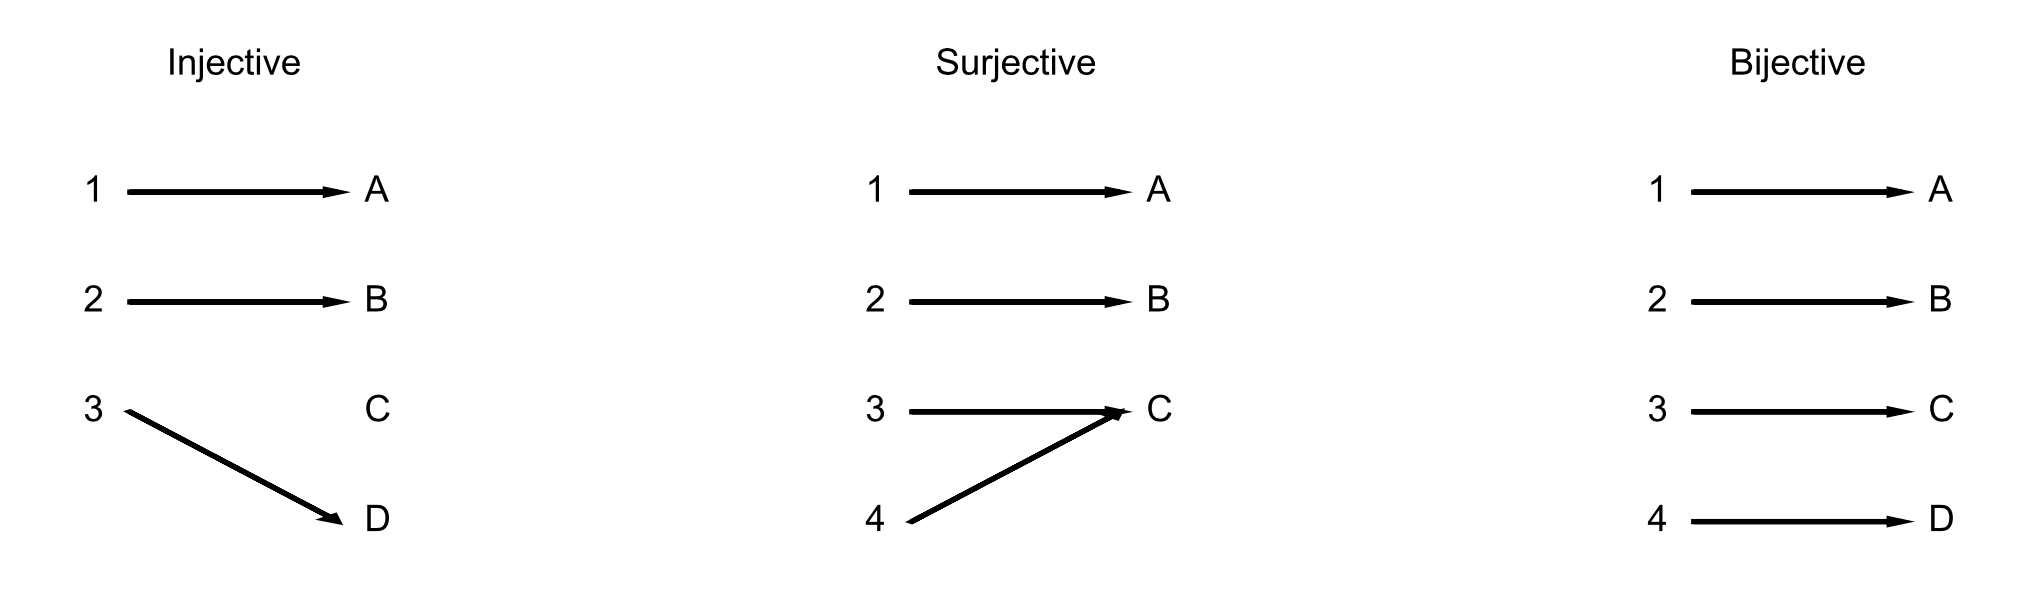
\includegraphics[width = 5in]{figures/mapping.png}
\end{figure}

\section*{Definition of Group}
\begin{definition}[Group]
    A group is a set plus an operation, that map an ordered pair of group element $(g,h)$ of $G$ into another element $g\cdot h \in G$, satisfying
    the following properties:
    \begin{enumerate}
        \item operation is associative: $g\cdot (h \cdot k) = (g\cdot h) \cdot k$ for $g,h,k \in G$;
        \item $G$ contain an identity element $e$, that satisfies $g\cdot e = e\cdot g = g$ for all $g \in G$ and 
        \item Each element of $G$ has an inverse, denoted by $g^{-1}$.
    \end{enumerate}  
\end{definition}

\subsection*{Order of the group}
    Order of the group $G$, or the cardinality of the group, is the number of elements in the set $G$, denoted by $|G|$
\vspace{-10pt} % reduce the space in successive definition
\subsection*{Abelian group}
    A group is called abelian if for all $g, h \in G$, $g\cdot h = h \cdot g$ (commutative)


\begin{definition}[Subgroup]
    Definition: $H$ is a non empty subset of $G$ and $H$ is a group, then $H$ is a subgroup of $G$
\end{definition}

\begin{theorem}
    The intersections of subgroups of $G$ is also a subgroup of $G$.
\end{theorem}
\begin{proof}
    Suppose $H$ and $L$ are subgroups of $G$. $M$ is the intersections between $H$ and $L$, then:
    \begin{enumerate}
        \item identity $e \in M$;
        \item if $h_1, h_2 \in H$ and $h_1 \cdot h_2 = e$, If $h_1\in L$, then inevitably $h_2 \in L$, therefore the intersections of $H$ and $L$ is closed under inverse;
        \item similarly, if $h_1, h_2 \in H$ and $h_1, h_2 \in L$, then $h_1\cdot h_2$ belong to both $H$ and $L$ are therefore in the intersections. $M$ is closed under group operation.
    \end{enumerate}
\end{proof}

\vspace{10pt}

\begin{definition}[Generator]
    For a set $S$, the intersections of all subgroups contain $S$ is a subgroup. This intersections is denoted by $\langle S\rangle$ and we say that it is generated by $S$. 
\end{definition}
For a group element $g$, we write that group that is generated by $g$ as $\langle g \rangle$, the order of $\langle g \rangle$ is also called the order of $g$. 

\subsection*{Cyclic group}
    If a group is generated by a single element, i.e. $G = \langle g \rangle$ for $g \in G$

\begin{theorem}
    if a group $G$ is finite, we must have $g^n = e$ for $g \in G$. Since any $g^a$ is a number in $G$
\end{theorem}


\section*{Two important group}

\subsection*{Linear transformation group}
Denoting $V$ as a vector space, we write $\text{GL}(V)$ as the group of all linear transformation in $V$

\subsection*{Permutation group}
Denoting a set by $X$. All the bijections of $X$ to itself form a group, which we denote $\Sym(X)$. 

If $|X| = n$, then $|\Sym(X)| = n!$.
If $|X| = |Y|$, then $\Sym(X) = \Sym(Y)$ and we denote it as $\Sym(n)$ or $S_n$.

We denote a permutation by $\pi\colon \{1,2,\dots,n\} \to \{ \cdots \}$. For example:
\[
    \pi = \left(  
    \begin{matrix} 
    1&2&3&4&5\\
    5&4&1&2&3
    \end{matrix}
    \right) \in S_5
\]
gives a permutation $\{1,2,3,4,5\} \to \{ 5,4,1,2,3 \}$. Such notation is called 'two-line notation'
We should note that the numbers are to be interpreted as indices of the objects in the set.
In matrix form, we have:
\begin{equation}
    \left( \begin{matrix} 5 \\ 4 \\ 1 \\ 2\\ 3 \end{matrix} \right)
    = \left( \begin{matrix} 
        0 & 0 & 0 & 0 & 1 \\
        0 & 0 & 0 & 1 & 0 \\
        1 & 0 & 0 & 0 & 0 \\
        0 & 1 & 0 & 0 & 0 \\
        0 & 0 & 1 & 0 & 0 
    \end{matrix} \right) 
    \left( \begin{matrix} 1 \\ 2 \\ 3 \\ 4 \\ 5 \end{matrix} \right)
\end{equation}
We call the matrix of permutation $A_{\pi}$. 
With the matrix notation, we can define the sign of a permutation:
\[\text{sign}\pi = \det A_{\pi}\]

\textbf{Cyclic notation}
For the example permutation $\{1,2,3,4,5\} \to \{ 5,4,1,2,3 \}$, we can simply write
$\pi = (153)(24)$
The interpretion of cyclic notation is as follows:
\begin{itemize}
    \item a cyclic is a permutation of a subset without affecting other elements,
    \item fixed point can be omitted,
    \item $(153)$ is read as $1\to 5, 5\to 3, 3\to 1$. $1\to5$ reads 'object in position 1 become object in position 5'.
\end{itemize}
We can generate the two-line notation from the cyclic notation as follows:
\begin{equation*}
    \begin{matrix}
                & 1 & 2 & 3 & 4 & 5 \\
        1 \to 5 \quad & 5 &   &   &   &   \\
        5 \to 3 \quad &   &   &   &   & 3 \\
        3 \to 1 \quad &   &   & 1 &   &   \\
        2 \to 4 \quad &   & 4 &   &   &   \\
        4 \to 2 \quad &   &   &   & 2 &   \\
                & 5 & 4 & 1 & 2 & 3
    \end{matrix}
\end{equation*}

The following arrow form of permutation is also convenient to keep track of the operation, especially for successive 
application of permutations. Note that the arrow $5\to1$ reads 'the object in position 5 is moved to position 1'.
\begin{figure*}[!h]
    \centering
    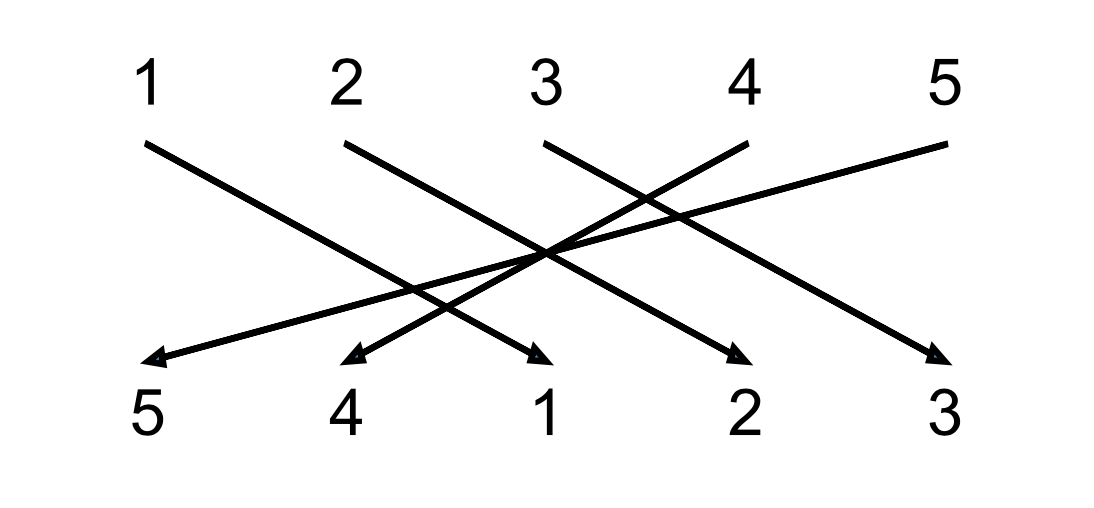
\includegraphics[width=2in]{figures/permutation_arrow.png}
\end{figure*}

Using cyclic notation, we can write $S_3 = \{ e, (1,2), (2,3), (1,3), (1,2,3), (3,2,1) \}$. We have $|S_3| = 6$. The group table of $S_3$ can be calculated 
and tabulated to be:
\begin{table}[h]
    \centering
    \caption{Multiplication table of $S_3$}
    \begin{tabular}{|c|ccc|ccc|}
        \hline
                & e     & (123) & (321) & (12)  & (13)  & (23)  \\ \hline
           e    & e     & (123) & (321) & (12)  & (13)  & (23)  \\ 
          (123) & (123) & (321) & e     & (13)  & (23)  & (12)  \\
          (321) & (321) & e     & (321) & (23)  & (12)  & (13)  \\ \hline
          (12)  & (12)  & (23)  & (13)  &     e & (321) & (123) \\
          (13)  & (13)  & (12)  & (23)  & (123) & e     & (321) \\
          (23)  & (23)  & (13)  & (12)  & (321) & (123) & e     \\ \hline
    \end{tabular}
    \label{T:s3}
\end{table}

\section*{Multiplication of group} 

\subsection*{Group multiplication}
For $S$ and $T$, both subset of group $G$, we define their product:
\begin{equation}
    ST = \{st\mid s\in S, t \in T\}
\end{equation}
and $sT \equiv \{s\}T $ and $Ts \equiv T\{s\} $ for $s \in S$.

\vspace{10pt}

\begin{definition}[Left cosets]
    For $H$ a subgroup of $G$ and $g \in G$, $gH$ is called a left coset. $Hg$ is called a right coset. 
    The set $\{gH \mid g \in G, H\ \text{is subgroup of}\ G\}$ is written as $G\setminus H$
\end{definition}

For example, for $S_3$ and its subgroup $H = \{e,(123),(132)\}$, 
Using the multiplication table \ref{T:s3}, we can find that
applying element $g \in \{(12), (23), (13)\}$ on $H$
give the set $\{(12), (23), (13)\}$. Therefore, the left cosets of $H$ is:
\[
    \left\{\, \{e,(123),(132)\}, \{(12), (23), (13)\}\, \right\}    
\]

\vspace{10pt}

\begin{theorem}
    The left cosets of the subgroup $H$ of $G$ partition $G$
\end{theorem}
\begin{proof}
    This is equivalent to say that $gH$ is either $H$ itself, or share no comment elements with $H$.
    if $g\in H$, then $gH = H$. On the other hand, 
    if $g\notin H$ but $gh \in H$ for an element $h\in H$, then, by the requirement of group $h^{-1}\in H$. $ghh^{-1} = g \in H$ which conflict with the assumption.
    Therefore, we $gH$ cannot share element with $H$: $|gH| = |H|$, so that left cosets of a subgroup partition the group.
\end{proof}
As a result, the whole group can be written as:
\[
    G = H + g_1 H + g_2 H + \dots + g_n H    
\]
\begin{theorem}[Lagrange's theorem]
    For a finite group $G$ and $H$ is a subgroup of $G$, $|H|$ can divide $G$.
\end{theorem}
\subsection*{Index of $H$ in $G$}
    The number of left cosets of a subgroup $H$ is called the index of $H$ in $G$, denoted as $[G:H]$.

If $G$ is a finite group and $g\in G$. Then the order of $\langle g\rangle$ divide $|G|$. This is because 
$\langle g\rangle$ is a subgroup of G.

\section*{Mapping}

\begin{definition}[Homomorphism]
    We define a mapping $\Phi\colon G \to H$ from group $G$ to $H$. If
    \[
        \Phi(g_1 g_2) = \Phi(g_1) \Phi(g_2)    
    \] 
    is satisfied for all $g_1, g_2 \in G$, then we call $\Phi$ a homomorphism
\end{definition}

\subsection*{Isomorphism}
    If the mapping $\Phi$ is a bijection, then we call $\Phi$ an isomorphism. If $G$ and $H$ are related by 
    an isomorphism, we write $G\cong H$

Isomorphic groups have the same group multiplication table, apart from the names or symbols and, if necessary, after 
rearranging rows and columns. 
With the aid of isomorphism, all groups can be subdivided into \emph{isomorphism classes} of isomorphic groups. 
Such a class is known as an \emph{abstract group}, each group within the isomorphism class are called 
\emph{realization of the abstract group}

\subsection*{Automorphism}
    We call the mapping $\Phi\colon G \to G$ (from $G$ onto itself) an automorphism

Automorphism are bijections. For example, $\Phi\colon G \to gG$ is an automorphism, 
this is shown in the rearrangement theorem. We write the set of all automorphism by $\Aut(G)$ 

\vspace{10pt}

\begin{theorem}[Rearrangement theorem]
    for group $G$ and a group element $g'\in G$, the set 
    \[\{g'g \mid g \in G\}\]
    contain each group element once and only once.
\end{theorem}
\begin{proof}
    It is equivalent to say that if $g_1 \neq g_2$, then $g'g_1 \neq g'g_2$. all group element in $G$ are mapped 
    to another distinct elements in $G$ (rearrangement).

    If $g'g_1 = g'g_2$ but $g_1 \neq g_2$, then 
    \[ g'^{-1}g'g_1 = g'^{-1}g'g_2 \] which apperant conflict with the assumption
\end{proof}

\vspace{10pt}

\begin{definition}
    [Kernel] For a homomorphism $\Phi\colon G \to H$, we define the kernel $\ker\Phi = \{g\in G\mid \Phi(g) = e_h \}$, i.\,e.\,,
    kernel of $\Phi$ is the elements in $G$ that are mapped to identity of group $H$. $\ker\Phi \subset G$
\end{definition}

\begin{definition}
    [Image] For homomorphism $\Phi\colon G \to H$, we define the image $\Image\Phi = \{ \Phi(g) \mid g \in G \}$, i.\,e.\,,
    the elements in $H$ that are obtained from the mapping. $\Image\Phi \subset H$
\end{definition}

\begin{lemma}
    $\ker\Phi$ is a subgroup of $G$
\end{lemma}
\begin{lemma}
    $\Image\Phi$ is a subgroup of $H$
\end{lemma}

\vspace{10pt}

\begin{theorem}
    Homomorphism $\Phi\colon G\to H$ is injective if and only if $\ker \Phi = e$
\end{theorem}
\begin{proof}
    If $\Phi$ is injective, then we require $\ker \Phi = e_g$; 

    If $\ker \Phi = e_g$. Suppose $\Phi(a) = h$ and $\Phi(b) = h$. If in group $G$, we have $ax = b$, with $x\in G$, 
    Then we have:
    \[  
        \Phi(b) = \Phi(a)\Phi(x)    
    \]
    This implies that $\Phi(x)=e_h$ and $x = e_g$. Therefore, $a = b$: if $\ker \Phi = e_g$ then we cannot have
    two different elements in $G$ that are mapped to the same element in $H$.
\end{proof}

\vspace{10pt}

\begin{definition}
    [Conjugation]
    We call the mapping $\Phi_g\colon G\to G$ with $\Phi_g(h) = ghg^{-1}$ a conjugation with $g$, or an \emph{inner conjugation}
\end{definition}
According to definition, $\Phi_g \in \Aut(G)$

\begin{definition}
    A subgroup is called normal, or self-conjugating, if every left cosets of $H$ in $G$ is also a right coset of $H$ in $G$
\end{definition}
If $H$ is a normal subgroup, then for the set $G/H$, we can show that $(g_1 H)\cdot(g_2 H)$ is also in 
set $G/H$:
\begin{proof}
    Since $H$ is a normal subgroup, by definition: 
    \[gH = Hg = gHg^{-1}g\] so that we fine:
    \[gHg^{-1} = H\]
    Then:
    \begin{align*}
        (g_1 H)\cdot(g_2 H) &= g_1 H g_1^{-1}g_1 g_2 H = H g_1 g_2 H \\
            &= (g_1g_2)(g_1g_2)^{-1} H (g_1g_2) H \\
            &= g_1g_2 H H = g_1 g_2 H 
    \end{align*}
    since $g_1 g_2 H$ is also a left coset and belong to $G/H$, we have shown that the set $G/H$ is indeed a group with 
    operation $(g_1 H)\cdot(g_2 H)$
\end{proof}

we call \textbf{quotinet group}, or factor group.
For example, for $H = \{e,(123),(132)\}$, we can verify that $H$ is a normal group, and the 
set ${H, (12)H}$ is a group with the defined operation.

\begin{lemma}
    The kernel $\ker\Phi$ of $\Phi\colon G\to H$ is a normal subgroup.
\end{lemma}

\begin{lemma}
    For a group homomorphism $\Phi\colon G\to H$, the quotinet group is isomorphic to $\Image\Phi$ (bijection).
\end{lemma}


\begin{definition}
    A group is called normal (self-conjugate) if 
    \[
        gBg^{-1} = B\ \text{for}\ g \in G \qquad \text{(group automorphism)}    
    \]
\end{definition}

% from crystall 
\begin{definition}
    [Conjugate classes]
    Two group elements $a$ and $b\in G$ are called conjugate if there is another element $g$, so that:
    \[g^{-1}ag = b\]
    The elements of $g$ can then be collected into classes. $C_k$, each is made of conjugate elements. 
\end{definition}
Conjugate partition $G$ into equivalent classes. $C_a = \{g^{-1}ag\mid g\in G\}$ is called conjugacy class 
from $a$

We have the following properties for conjugation:
\begin{enumerate}
    \item every element in $G$ belongs to exactly one conjugacy class,
    \item the numbers of elements in conjugacy classes are different, but they are always divisor of order of $G$,
    \item If for $g_i\in G$ and we have $gm^{-1}g_i g_m = g_i$ for all $g_m \in G$, then $g_i$ is called self-conjugate. 
    \item For abelian group, all its elements is self-conjugate, and thus form a conjugacy class by itself,
    \item Elements in the same conjugacy class have the same order.
\end{enumerate}

Two subgroup $H$ and $H'$ are called conjugate subgroups in $G$ if there exist an element $g_m\in G$
so that $H' = g_m^{-1}Hg_m$. The set of subgroups that are conjugate to $H$ for a conjugacy class. 

The conjugate subgroups are isomorphic and have the same order. If for a subgroup $H$ in $G$, $g_m^{-1}Hg_m = H$
for all $g_m \in G$, Then $H$ is a normal subgroup


\section*{Action of a group}

\begin{definition}
    [Action of a group]
    For a group $G$ and a set $\setM$, the action of $G$ on $\setM$ is a mapping 
    $\alpha\colon G\times \setM \to \setM$ satisfying:
    \begin{enumerate}
        \item $\alpha(e,m) = m$ for $m \in \setM$;
        \item $\alpha(g, \alpha(h,m)) = \alpha(gh, m)$ for $m\in \setM$ and $h,g\in G$
    \end{enumerate}
\end{definition}
where $\alpha(g,m)$ means action of a group element $g$ on a set element in $\setM$

For an action $\alpha$, we have a homomorphism that map group $G$ to permutation group on $\setM$, 
given by:
\[g\to (m\to \alpha(g,m))\]
$m\to \alpha(g,m)$ being a permutation. 

\subsection*{Group action on itself}
For a group $G$, $G$ can act on itself by conjugation: $\alpha\colon G\times G \to G$ given by
$\alpha(h,g) = hgh^{-1}$

\vspace{10pt}

\begin{definition}
    [Orbit under $G$]
    For $G$ acting on $\setM$, the sets $Gm = \{gm\mid g\in G\}$ partition the set $\setM$. 
    \[\setM = Gm_1 + Gm_2 + \dots + Gm_n\]
    Each set $Gm$ is called the orbit of $m$ under $G$.
\end{definition}

\subsection*{Transitive}
An action is called transitive if it has only one orbit

\begin{definition}
    [Symmetry]
    For a group $G$ acting on $\setM$, $T\subset M$ is called invariant under $S \subset G$ if $ST\subset T$, 
    with $ST = {\alpha(g,m)\mid g \in G, m\in T}$. 
    The elements in $S$ are called 'symmetry'.
\end{definition}

\subsection*{Stabilizer}
For group $G$ acting on $\setM$ and $m \in \setM$, the set 
\[G_m = \{ g\in G\mid gm = m \}\]
are called the stabilizer of $m$. $G_m \subset G$

\begin{lemma}
    $G_m$ is a subgroup of $G$, $|G_m|$ divide $G$. Further more, $G_m$ is a normal subgroup. 
    The mapping $f\colon Gm \to G/G_m$ is a bijection and $|G|=|G_m||Gm|$
\end{lemma}

\section*{Isometry}

\begin{definition}
    [Isometry]
    The distance in euclidean space is given by 
    \[
        d(x,y) = \sqrt{\sum_i(x_i-y_i)^2}    
    \]
    A mapping $g\colon \mathbb{R}^n \to \mathbb{R}^n$ satisfying 
    \[
        d(g(x),g(y)) = d(x,y)    
    \] is called an isometry, the transformation that keep the distance. We denote them as $\AO(n)$ or $\E(n)$
\end{definition}
The group of all isometries is a subgroup of permutation between points in n-dimensional space $\Sym(\mathbb{R}^n)$

\subsection*{Translation}
with $x, a \in \mathbb{R}^n$, transformation $t_a\colon x \to x+a$ is called translation.

\subsection*{Orthogonal linear map}
An orthogonal linear map is a linear transformation that perserve the inner product, the group of all
orthogonal linear map is denoted as O($3$)

\begin{theorem}
    For any group element $g\in \AO(n)$ (isometry), there exist a unique pair $(a,r)$ such that 
    \[g = t_a \cdot r\]
    with $r\in \AO(n)$ that fix the point at origin (rotation). $r$ is a anorthogonal linear map
\end{theorem}
As a result, any isometry is an orthogonal linear map followed by translation.

\vspace{10pt} %%%%%%%%%%%%%%%%%%%%%%%%%%%%%%%%%%%%

For a subgroup $G\subset \AO(n)$, the map $R\colon G \to R(G)$ with $R(G)\in \text{O}(n)$ given by
$g = t_a R(g)$ is a group homomorphism. It's kernel is $T(G)$:
\begin{equation}
    T(G) = \{ a \in \mathbb{R}^n \mid t_a \in G\}
\end{equation}
the set of all translation. 

\begin{lemma}
    $T(G)$ is invariant under $R(G)$
\end{lemma}
i.\,e.\,, the application of $r\in R(G)$ on $t\in T(G)$ gives another translation in $T(G)$

\vspace{10pt} %%%%%%%%%%%%%%%%%%%%%%%%%%%%%%%%%%%%

\begin{definition}
    [Lattice]
    a discrete subgroup of $\mathbb{R}^n$ is called Lattice (with $+$ as group operation). The dimension of its span is called rank.
\end{definition}
Let $a_1,\dots,a_k \in \mathbb{R}^n$ be linearly independent, then the set 
$L = \sum_i \mathbb{Z} a_i$ is a lattice.

A subgroup $G\subset \AO(n)$ act discretely if all orbits in $\mathbb{R}^n$ is discrete.

\begin{lemma}
    If $G$ is a subgroup of $\AO(n)$ leaving a lattice $T$ invariant, then $G$ is finite
\end{lemma}

\begin{definition}
    [Crystallographic group]
    If $G$ is a subgroup of $\AO(n)$ for which $T(G)$ is the lattice translation, then $G$ is called 
    a crystallographic group.
\end{definition}
\subsection*{Crystallographic point group}
If $G\subset \text{O}(n)$ leave invariant a lattice of rank $n$, then $G$ is called a crystallographic point group

\begin{lemma}
    If $G$ is a crystallographic group, then $R(G)$ is a crystallographic point group
\end{lemma}


\newpage
\part{Crystal Structure}
\section*{Definitions}
We consider a \emph{crystal structure} as the following object:
\begin{definition}
    [Crystal Pattern]
    The infinite, three-dimensional periodic array corresponding to a crystal is called \emph{crystal pattern}.
    The lengths of the periodicity may not be arbitrarily small. Crystal pattern is also known 
    as \emph{infinite ideal crystal}.
\end{definition}
We further distinguish two other concepts:
\begin{itemize}
    \item \emph{Macroscopic crystal} is a finite block of a crystal pattern,
    \item \emph{real crystal} has a finite size, but also defects.
\end{itemize}

\subsection*{Translation}
A shift which bring the crystal structure to superposition with itself is called 
a \emph{symmetry translation} or simply translation for this crystal structure. 
It is specified by a translation vector.

\vspace{10pt}

\begin{definition}
    [Vector lattice]
    The infinite set of all translation vectors $\bft_i$ of a crystal pattern is its \emph{vector lattice} $\mathbf{T}$, 
    or simply the \emph{lattice}. 
    The vectors are called \emph{lattice vectors}
\end{definition}
We distinguish vector lattice from the following two concepts:

\subsection*{Point lattice}
Choosing a starting point $\bfx_0$, the set of all the end points $\{\bfx_i\mid\bfx_i = \bfx_0 + \bft_i\}$
is call the \emph{point lattice} belongs to $\bfx_0$ and $\mathbf{T}$.
\subsection*{Particle lattice}
If the chosen point of a point lattice correspond to center of gravity of particles. Then we call this point lattice \emph{particle lattice}

The points that are related by translations are called \emph{translation equivalent}.

\vspace{10pt}

\subsection*{Basis}
To describe position in three-dimensional space, we need to choose an origin and a basis. 
A basis that consists of three lattice vectors of a crystal pattern is called a \emph{crystallograhic basis}
or a \emph{lattice basis} of the crystal structure. 

We further define the following terms:
\begin{itemize}
    \item \emph{Conventional basis} are the crystallograhic basis used in the International Tables A.
    \item \emph{Primitive basis} are the basis $a$, $b$ and $c$ with which every lattice vector $\bft$ can be expressed 
            as a linear combination with integral coefficients: $\bft = t_1 a + t_2 b + t_3 c$
\end{itemize}
A lattice is called \emph{primitive} if its conventional basis is primitive,  otherwise, we call it \emph{centred}. 

\subsection*{Unit cell}
A region in which all the points have coordinates \[0 \leq x,y,z < 1\]
with respect to its chosen basis and origin is called a \emph{unit cell} of the crystal structure.

\vspace{10pt}

\section*{Symmetry operations}
\begin{definition}
    [Symmetry operation]
    A symmetry operation is a mapping of an object such as 1) all distances remain unchanged and 2) the obejct is mapped onto itself or its mirror image.
    If the obejct is a crystal structure, the mapping is called a \emph{crystallographic symmetry operation}.
\end{definition}

\subsection*{Space group}
The set of all symmetry operations of a crystal structure is called the space group of the crystal structure.

\vspace{10pt}

\begin{definition}
    [Affine mapping]
    A mapping of space which maps parallel straight lines onto parallel straight lines is called an affine mapping. They do not necessary perserve 
    distance or angles.
\end{definition}

After choosing a coordination system, an affine mapping can always be represented as:
\begin{equation}
    \left( \begin{matrix}
        a'\\b'\\c'
    \end{matrix} \right)  = \left( \begin{matrix}
        w_{11} & w_{12} & w_{13} \\
        w_{21} & w_{22} & w_{23} \\
        w_{31} & w_{32} & w_{33}
    \end{matrix} \right) \left( \begin{matrix}
        a\\b\\c
    \end{matrix} \right)+ \left( \begin{matrix}
        w_1\\w_2\\w_3
    \end{matrix} \right)
\end{equation}
or simply, in matrix notation $\bfx' = W\bfx + w$. Affine mapping are Linear transformations.

\subsection*{Fixed point} A point $\bfx_F$ that is mapped onto itself is called a fixed point of the mapping.

\vspace{10pt}

\begin{definition}
    [Isometry]
    An affine mapping that leaves all distances and angles unchanged is called \emph{isometry}
\end{definition}
For an affine mapping to be an isometry, we require: 
\begin{enumerate}
    \item $\det W = \pm 1$ and 
    \item the matric tensor $G$ remain unchanged.
\end{enumerate}
where the matric tensor are a set of coefficients:
\begin{equation}
    G = \left(\begin{matrix}
        a^2 & ab\cos\gamma & ac\cos\beta \\
        ab\cos\gamma & b^2 & bc\cos\alpha \\
        ac\cos\beta & bc\cos\alpha & c^2 
    \end{matrix}\right)
\end{equation}
from the \emph{lattice parameter} $a$, $b$, $c$, $\alpha$, $\beta$ and $\gamma$

\vspace{10pt}

\subsection*{Types if isometries}
We can distinguish the following kinds of isometries in space:
\begin{enumerate}
    \item identity $\mathbf{I}$
    \item translation $\mathbf{T}$
    \item rotation and screw rotation $\mathbf{R}$
    \item inversion $\bar{\mathbf{I}}$
    \item rotoinversion $\overline{\mathbf{R}} = \bar{\mathbf{I}} \mathbf{R} = \mathbf{R} \bar{\mathbf{I}}$
    \item Reflection or glide reflections
\end{enumerate}
The symmetry operations satisfying \[\det W = -1\] are called the symmetry operation of the second kind.

\vspace{10pt}

\section*{Space groups and point groups}
\subsection*{Molecular symmetry}
The symmetry of a molecular (finite cluster of atoms) froms a group which is called the \emph{point group} $P_M$ of the molecule. $P_M$
can be infinite if the molecular is linear (infinite rotations). 

If we consider an ideal molecular to have translational symmetry in one direction, its symmetry group is called \emph{Rod group}, 
For translational symmetry in two dimension, it is called \emph{layer group}.

Two molecular point group belong to the same point group type if, after a change of basis, the transformation matrix of the two point group
coincide. 

\vspace{10pt}

\begin{definition}
    [Site symmetry]
    A point in a molecule has a definite site symmetry $S$ (site symmetry group) consists of all symmetry operations of the point group
    of the molecule that leave the point fixed. They correspond to stabilizer of the point in $G$.
\end{definition}

\subsection*{General position}
A set of symmetrically equivalent points $X$ of a molecular is in a \emph{general position} if the site symmetry $S$ of the point
consists of only identity. 
Otherwise, the points are in a \emph{special position}

For a point $X_s$ having site symmetry $S$, there exist $|P_M|/|S|$ symmetrically equivalent points. 
The length of the orbital is called its multiplicity.
The multiplicity of a point in the general position is the order of the molecular group $P_M$.

\begin{definition}
    [length of the orbital]
    For a finite group $G$ and stabilizer of the element $m$, then $L = |G|/|S|$ is the length of the orbital $G_m$
\end{definition}

\begin{definition}
    [Wyckoff position]
    Two orbitals of $P_M$ $O_1$ and $O_2$ belong to the same Wyckoff position if, after having selected two arbitrary points $X_1 \in O_1$ 
    and $X_2 \in O_2$, Their site symmetry $S_1$, $S_2$ are conguate in $P_M$: there exist a symmetry operation $g \in P_M$ so that:
    \[S_2 = g^{-1}S_1 g\]
\end{definition}

\vspace{10pt}

\begin{definition}
    [Point group of crystal structure]
    The point group of a crystal structure is the symmetry group of the bundle of vectors that is normal to the face of crystal.
\end{definition}
Here, the face refer to the surface of idealy grown crystal (crystal growth involves parallel advancement of crystal faces). 
The point group of crystal structure is therefore the symmetry of vectors, and the symmetry operation involve only 
the matrix part $W$ and is finite

\begin{lemma}
    Translation groiup $T$, the set of all translations of a space group $G$,sis a normal subgroup of $G$.
\end{lemma}
The coset decomposition of $G$ with respect to $T$ contain exactly those elements which has the same matrix part. 
Therefore, every matrix $W$ is characteristic for the corresponding cosets. 

\begin{lemma}
    The factor group $G/T$ is isomorphic to the point group $P$ of the crystal.
\end{lemma}

\vspace{10pt}

\section*{Classification of space groups}
\begin{definition}
    [Crystal class]
    Two crystallograhic point groups $P_1$ and $P_2$ belong to the same point group type, if a basis can be found 
    so that the matrix part of $P_1$ and $P_2$ coincide. We say that they belong to the same \emph{Crystal class}
\end{definition}
There are 32 crystal class in space and 10 in plane.
Amoung the 32 crystal class, there are seven that belong to the point groups of the lattice. The seven point groups 
are called \emph{holohedries}. We can assign the points groups to holohedries as:
\begin{enumerate}
    \item The point group of the crystal class $P$ is a subgroup of that of the holohedry $H$,
    \item the index $H/P$ is as small as possible
\end{enumerate}
The seven holohedries assigned to the space groups are called the \emph{crystal systems} of space groups

\vspace{10pt}

\begin{definition}
    [Affine space group types]
    Two space groups $G_1$ and $G_2$ is said to belong to the same affine space group types if 
    all their matrix-column pairs $\{(W,w)\}$ coincide with an appropriately chosen basis vectors. 
\end{definition}
They belong to the same \emph{crystallograhic space group types} if 
all their matrix-column pairs $\{(W,w)\}$ coincide with an appropriately chosen right-handed coordination system.

There are 219 affine space group types and 230 space group types. 
We distinguish space groups and space group types. Therefore 230 different space group types, but there are 
infinite space groups in a space group types, one for each crystal structure.

\begin{definition}
    [Bravais type]
    Two point lattice belong to the same bravais type if their space groups belong to the same space-group type.
\end{definition}

\vspace{10pt}

\emph{Site symmetry group} $S_x$ for space group $G$ has the same definition of that in molecular: it is 
a subgroup of $G$ that leave $x$ unchanged. 
If $g\in G$ is a site symmetry of $x$, then $g' = tgt^{-1}$ is a site symmetry of $tx$:
\begin{equation}
    g'tx = tgx = tx
\end{equation}

The number of symmetry equivalent points of a general position in a primitive cell is equal to the point 
group of the crystal structure $P$ because point group is isomorphic to the factor group $G/T$

Every site-symmetry group $S$ of a space group $G$ is isomorphic to a subgroup of the point group $P$ of $G$. 
For general position, $S$ is isomorphic to $P$, their multiplicity is given by $|P|/|S|$ or equivalently $|G/T|/|S|$.

\section{Subgroups and Supergroups of point and space group}
\begin{definition}
    [Translationengleiche subgroup]
    $H$ is called an \emph{Translationengleiche subgroup} of $G$ if $H$ and $G$ have the same group of translation. 
    Therefore, $H$ belongs to a crystal class of lower symmetry than $G$: $P_H < P_G$
\end{definition}

\begin{definition}
    [Klassengleiche subgroup]
    $H$ is called an \emph{Klassengleiche subgroup} of $G$ if $H$ and $G$ belong to the same crystal class. 
    Therefore, $H$ has fewer translations than $G$: $T_H < T_G$
\end{definition}

\subsection*{General subgroup}
$H$ is called a general subgroup if $T_H < T_G$ and $P_H < P_G$

A klassengleiche subgroup is called an isomorphic subgroup if $G$ and $H$ belong to the same affine space-group type. 
For an isomorphic subgroup, we have the following:
\begin{enumerate}
    \item isomorphic subgroup $H$ in general belong to the same space group types with $G$, or its enantiomorphic partner (left-handed correspondence).
    \item The basis vectors are changed so that all symmetry elements are changed,
    \item Symmetry are lowered, since symmetry operations (translation) are lost, however, the two space groups $G$ and $H$ are isomorphic.
\end{enumerate}

\begin{theorem}
    [Theorem of Hermann]
    A maximal subgroup of a space group is either translationengleiche or klassengleiche.
\end{theorem}

\vspace{10pt}

\begin{definition}
    [Supergroup]
    If $H$ is a maximal translationengleiche, klassengleiche or isomorphic subgroup of $G$, then $G$
    is the minimum translationengleiche, klassengleiche or isomorphic supergroup of $H$.
\end{definition}


\newpage
\part{Representation Theory}

\section*{Representation}

\begin{definition}
    [Representation]
    A linear representation of a group $G$ on vector space $V$ is a homomorphism:
    \[\rho\colon G\to \GL(V)\]
\end{definition}
We define the following terms:
\begin{itemize}
    \item $G$ \emph{act linearly} on $V$,
    \item $V$ is called a \emph{G-module},
    \item Dimension of the representation is the dimension of the vector space $V$, and
    \item $(g,v)=\rho(g)v$ is an action of $g\in G$ on $v\in V$ 
\end{itemize}
If the homomorphism $\rho$ from group elements to linear transformation is a injective, 
it is called \emph{faithful}.

\subsection*{Regular representation}
For a group $G$ of order $n$ and an $n$-dimensional vector space with corresponding basis vector 
$\{e_{g_1},\dots,e_{g_n}\}$ (each group element correspond to a basis vector), then, 
we call a representation $\rho\colon G\to \GL(V)$ with $\rho(g_i) e_{g_j} = e_{g_i g_j}$
as \emph{regular representation}

\vspace{10pt}

\begin{definition}
    [Interwine]
    If $r$ and $s$ are representation of $G$ on vector space $V$ and $W$, then a map
    $T\colon V\to W$ interwine $r$ and $s$ if:
    \[s(g)T = Tr(g) \qquad g\in G\]
\end{definition}
We call the mapping $T$ as a \emph{homomorphism of G-module} $V\to W$. The set of all such homomorphism of G-module 
between $V$ and $W$ are denoted as $\Hom_G(v,W)$

\subsection*{Equivalent representation}
Representation $r$ and $s$ are called equivalent if there is a linear isomorphism $T\colon V\to W$ that 
interwine $r$ and $s$.

We further call all such linear isomorphism \emph{isomorphism of G-modules} 

\vspace{10pt}

\subsection*{Sub-G-Module}
For $r$ a representation of $G$ on $V$, $W\subseteq V$, a subspace of $V$ is invariant if 
$r(g)w \in W$ for all $g\in G$. 
In this case, we have a \emph{subrepresentation} of $G\to \GL(W)$ and $W$ is called 
\emph{sub-G-module of V}

Suppose $G$ is finite and $\rho$ is a representation of $G$ on $V$ and $U$ is a sub-G-module of $V$,
then, there exist a sub-G-module $W$ of $V$ so that $V$ is given by a direct sum of $U$ and $W$:
\[V = U \oplus W\]

\begin{definition}
    [Reducible]
    A G-module $V$ is reducible if it has sub-G-module other than $0$ (the origin) and itself. 
    Otherwise, it is called \emph{irreducible}.
\end{definition}
If $V$ is the direct sum of irreducible sub-G-modules, then $V$ is called \emph{completely reducible}.
(A representation is reducible if its matrix representation can be written in block diagonal form.)

\begin{lemma}
    For a finite group $G$, every finite-dimensional G-modules is completely reducible.
\end{lemma}

\end{document}
